\section{最优性与导数计算}
\label{sec:mfo-optimality}

普通的判据$\nabla f=\bm{0}$在球面上失效：在极小点$\bm{e}_1$处，$\nabla f$等于$\bm{e}_1$，并不为零。约束下应该把哪个量算成零，怎样判别二阶情形，这些量在具体约束上怎样计算？

\paragraph{切向梯度}
黎曼度量的作用之一是把微分变成向量：$\operatorname{grad}f(\bm{x})$是$T_{\bm{x}}M$中满足下式的唯一向量，$\mathrm{d}f_{\bm{x}}$是$f$在$\bm{x}$处的微分。
\begin{equation}
 \langle\operatorname{grad}f(\bm{x}),\bm{v}\rangle_{\bm{x}}=\mathrm{d}f_{\bm{x}}[\bm{v}],
 \qquad\forall\,\bm{v}\in T_{\bm{x}}M.
 \label{eq:mfo-riem-grad-def}
\end{equation}
这个向量称为\term{黎曼梯度}（Riemannian gradient）。微分和度量的具体定义见\BookChapterRef{chap:manifold-calculus}{卷四第28章“流形上的微积分”}，这里只用它的计算结果。

度量如何影响梯度？设切空间上的内积由对称正定矩阵$\bm{G}$给出，微分的系数向量记为$\bm{c}$。式~\eqref{eq:mfo-riem-grad-def}化成
\[
 \bm{v}^\top\bm{G}\operatorname{grad}f=\bm{v}^\top\bm{c},\qquad\forall\,\bm{v},
\]
于是
\[
 \operatorname{grad}f=\bm{G}^{-1}\bm{c}.
\]
取$\bm{c}=(1,1)^\top$做比较。$\bm{G}=\bm{I}$时梯度是$(1,1)^\top$；$\bm{G}=\operatorname{diag}(4,1)$时梯度是$(\tfrac14,1)^\top$。

图~\ref{fig:mfo-metric-gradient}解释这个差别。绿色区域是该度量下的单位球，梯度方向指向单位球上使线性函数最大的那一点。度量把单位球压扁，切点就移动了。两种度量下，梯度为零的条件都是$\bm{c}=\bm{0}$，所以驻点不受影响。

\begin{BookInlineFigure}
 \centering
 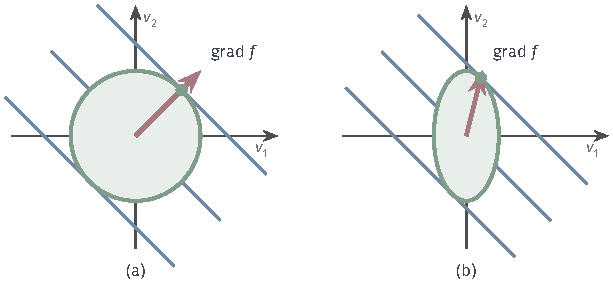
\includegraphics[width=103.8mm]{figures/05-optimization/06-constrained-optimization/tikz/mfo-metric-gradient/figure.pdf}
 \caption{同一微分在两种度量下的梯度。蓝线是线性函数$\mathrm{d}f[\bm{v}]=v_1+v_2$的等值线，绿色区域是度量的单位球，绿点是单位球上函数值最大的点，红箭头是梯度。(a)~$\bm{G}=\bm{I}$。(b)~$\bm{G}=\operatorname{diag}(4,1)$，单位球沿$v_1$被压缩，梯度偏向$v_2$。}
 \label{fig:mfo-metric-gradient}
\end{BookInlineFigure}

\paragraph{诱导度量下用投影计算}
取诱导度量时，黎曼梯度有一个直接的算法。设$\bar{f}$是$f$在环境空间中的光滑延拓，$\bm{P}_{\bm{x}}$是到$T_{\bm{x}}M$的正交投影。下面的引理说明，只要把欧氏梯度投影一下。

\begin{lemma}[投影公式]
 \label{lem:mfo-projection-gradient}
 设$M\subseteq\mathbb{R}^n$是嵌入子流形，取诱导度量，$\bar{f}$在$M$的邻域内光滑且在$M$上等于$f$。则
 \begin{equation}
  \operatorname{grad}f(\bm{x})=\bm{P}_{\bm{x}}\nabla\bar{f}(\bm{x}).
  \label{eq:mfo-projection-gradient}
 \end{equation}
\end{lemma}

\begin{proof}
 对$\bm{v}\in T_{\bm{x}}M$，取$M$上的曲线$\bm{c}$，满足$\bm{c}(0)=\bm{x}$，$\bm{c}'(0)=\bm{v}$。因为$f$与$\bar{f}$在$M$上相等，
 \[
  \mathrm{d}f_{\bm{x}}[\bm{v}]=\frac{\mathrm{d}}{\mathrm{d}t}\bar{f}(\bm{c}(t))\Big|_{t=0}=\langle\nabla\bar{f}(\bm{x}),\bm{v}\rangle.
 \]

 $\bm{P}_{\bm{x}}$是正交投影，$\bm{v}$在切空间中，所以$\bm{P}_{\bm{x}}\bm{v}=\bm{v}$，并且投影对称，于是
 \[
  \langle\nabla\bar{f}(\bm{x}),\bm{v}\rangle=\langle\nabla\bar{f}(\bm{x}),\bm{P}_{\bm{x}}\bm{v}\rangle=\langle\bm{P}_{\bm{x}}\nabla\bar{f}(\bm{x}),\bm{v}\rangle.
 \]
 $\bm{P}_{\bm{x}}\nabla\bar{f}(\bm{x})$在切空间中，又满足定义式~\eqref{eq:mfo-riem-grad-def}，由唯一性得结论。
\end{proof}

投影公式的适用条件是诱导度量，这一点不能省略。换了别的度量，还须按上一段的公式乘以度量的逆。

\paragraph{球面Rayleigh商}
把公式用到贯穿例。球面上的投影去掉沿$\bm{x}$的分量：
\[
 \bm{P}_{\bm{x}}\bm{z}=\bm{z}-(\bm{x}^\top\bm{z})\bm{x}.
\]

记\term{Rayleigh商}（Rayleigh quotient）的取值为$q(\bm{x})=\bm{x}^\top\bm{A}\bm{x}$，这里$\lVert\bm{x}\rVert_2=1$。欧氏梯度是$\bm{A}\bm{x}$，$\bm{x}^\top\bm{A}\bm{x}=q$，所以
\begin{equation}
 \operatorname{grad}f(\bm{x})=\bm{A}\bm{x}-q(\bm{x})\bm{x}.
 \label{eq:mfo-rayleigh-grad}
\end{equation}

在起点$\bm{x}^{(0)}$上算一遍。先算下面三个量：
\[
 \bm{A}\bm{x}^{(0)}=\frac13(2,4,4)^\top,\qquad q(\bm{x}^{(0)})=\frac{4+8+4}{9}=\frac{16}{9}.
\]
代入式~\eqref{eq:mfo-rayleigh-grad}，得到
\[
 \bm{g}^{(0)}=\frac13(2,4,4)^\top-\frac{16}{27}(2,2,1)^\top=\frac{1}{27}(-14,4,20)^\top.
\]

可以检查它在切空间中：$\bm{x}^{(0)\top}\bm{g}^{(0)}=(-28+8+20)/81=0$。范数的平方是
\[
 \lVert\bm{g}^{(0)}\rVert_2^2=\frac{196+16+400}{729}=\frac{68}{81}.
\]

图~\ref{fig:mfo-tangent-projection}画出这次分解。蓝色的欧氏梯度分成两段，紫色部分沿法向，只会改变到球面的距离，绿色部分才对球面上的运动起作用。

\begin{BookInlineFigure}
 \centering
 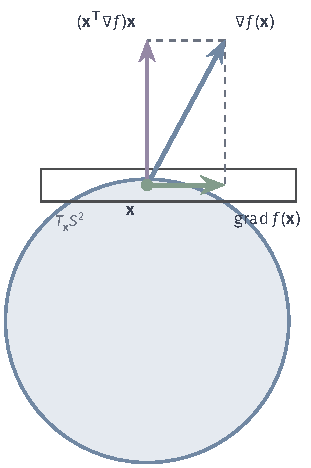
\includegraphics[width=52.7mm]{figures/05-optimization/06-constrained-optimization/tikz/mfo-tangent-projection/figure.pdf}
 \caption{起点$\bm{x}^{(0)}$处欧氏梯度的分解。蓝箭头是$\nabla f$，紫箭头是法向分量，绿箭头是切向分量即黎曼梯度，方框是切平面的一块。三个箭头按同一比例缩短到原长的$0.6$倍。}
 \label{fig:mfo-tangent-projection}
\end{BookInlineFigure}

\paragraph{一阶条件与Lagrange乘子}
现在把切向梯度与第~\ref{chap:constrained-optimality}章的乘子联系起来。由式~\eqref{eq:mfo-tangent}，$T_{\bm{x}}M$的正交投影可以写成
\[
 \bm{P}_{\bm{x}}=\bm{I}-\bm{J}^\top(\bm{J}\bm{J}^\top)^{-1}\bm{J},
\]
这里行满秩保证$\bm{J}\bm{J}^\top$可逆。

把投影代入式~\eqref{eq:mfo-projection-gradient}，并定义乘子
\begin{equation}
 \bm{\nu}(\bm{x})=-(\bm{J}\bm{J}^\top)^{-1}\bm{J}\nabla\bar{f}(\bm{x}),
 \label{eq:mfo-ls-multiplier}
\end{equation}
就得到
\begin{equation}
 \operatorname{grad}f(\bm{x})=\nabla\bar{f}(\bm{x})+\bm{J}(\bm{x})^\top\bm{\nu}(\bm{x})=\nabla_{\bm{x}}\mathcal{L}(\bm{x},\bm{\nu}(\bm{x})).
 \label{eq:mfo-grad-lagrange}
\end{equation}
所以黎曼梯度正是Lagrange函数对$\bm{x}$的梯度，乘子取使$\lVert\nabla\bar{f}+\bm{J}^\top\bm{\nu}\rVert_2$最小的最小二乘乘子。黎曼梯度为零，就是Lagrange乘子驻定条件。

球面上$h(\bm{x})=\bm{x}^\top\bm{x}-1$，$\bm{J}=2\bm{x}^\top$，$\bm{J}\bm{J}^\top=4$，代入式~\eqref{eq:mfo-ls-multiplier}得到
\[
 \nu(\bm{x})=-\frac14\cdot2\bm{x}^\top\bm{A}\bm{x}=-\frac12q(\bm{x}).
\]
梯度为零的条件$\bm{A}\bm{x}=q\bm{x}$说明，驻点恰好是$\bm{A}$的单位特征向量，并且$q$就是特征值。贯穿例有六个驻点$\pm\bm{e}_1,\pm\bm{e}_2,\pm\bm{e}_3$。

图~\ref{fig:mfo-rayleigh-landscape}是目标在球面上的等高线。红点$\bm{e}_1$周围的闭合曲线表明这里是极小点，$\bm{e}_3$是极大点，$\bm{e}_2$处等高线呈交叉状，它是鞍点。

\begin{BookInlineFigure}
 \centering
 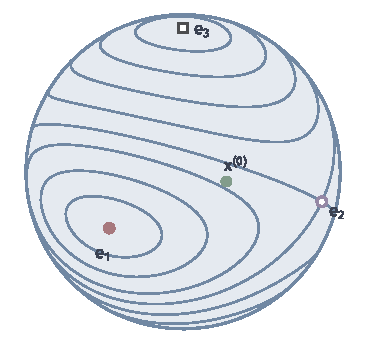
\includegraphics[width=62.0mm]{figures/05-optimization/06-constrained-optimization/matplotlib/mfo-rayleigh-landscape/figure.pdf}
 \caption{贯穿例的目标在单位球面上的等高线（蓝），只画朝向读者的半球。红点是极小点$\bm{e}_1$，紫圈是鞍点$\bm{e}_2$，方块是极大点$\bm{e}_3$，绿点是起点。背面半球的$-\bm{e}_1,-\bm{e}_2,-\bm{e}_3$有相同的情形。}
 \label{fig:mfo-rayleigh-landscape}
\end{BookInlineFigure}

\paragraph{切向曲率}
一阶条件分不开$\bm{e}_1,\bm{e}_2,\bm{e}_3$，需要二阶信息。\term{黎曼Hessian}（Riemannian Hessian）是切空间$T_{\bm{x}}M$到自身的对称线性算子，记为$\operatorname{Hess}f(\bm{x})$，定义为黎曼梯度沿切向量的协变导数，其几何来历可参考\BookChapterRef{chap:riemannian-geometry}{卷四第27章“黎曼几何”}。

诱导度量下的协变导数是先做普通方向导数再投影，所以只要把黎曼梯度光滑延拓成环境空间中的向量场$\bm{G}$，就有
\begin{equation}
 \operatorname{Hess}f(\bm{x})[\bm{v}]=\bm{P}_{\bm{x}}\,\mathrm{D}\bm{G}(\bm{x})[\bm{v}].
 \label{eq:mfo-hess-projection}
\end{equation}

球面上把式~\eqref{eq:mfo-rayleigh-grad}的右端在整个空间中当作$\bm{G}(\bm{x})$，方向导数是
\[
 \mathrm{D}\bm{G}(\bm{x})[\bm{v}]=\bm{A}\bm{v}-2(\bm{x}^\top\bm{A}\bm{v})\bm{x}-q(\bm{x})\bm{v}.
\]
第二项沿法向，投影后消失；第三项本身是切向的。于是
\begin{equation}
 \operatorname{Hess}f(\bm{x})[\bm{v}]=\bm{P}_{\bm{x}}\bigl(\bm{A}\bm{v}\bigr)-q(\bm{x})\bm{v},\qquad \bm{v}\perp\bm{x}.
 \label{eq:mfo-rayleigh-hess}
\end{equation}

这个式子里的$-q\bm{v}$值得留意。欧氏Hessian是$\bm{A}$，而切向曲率还要减去$q$，这一项来自约束本身的弯曲，由乘子项承担，下面马上看到。

在驻点上用这个公式。取$\bm{x}=\bm{e}_i$，$q=\lambda_i$，切空间由其余两个坐标向量张成，算子是对角的。三个驻点的切向曲率如表~\ref{tab:mfo-critical}所示。

\begin{BookInlineTable}
 \centering
 \caption{贯穿例的驻点，切向曲率由式~\eqref{eq:mfo-rayleigh-hess}算出。}
 \label{tab:mfo-critical}
 \begin{tabular}{llll}
  \toprule
  驻点 & $q$ & 切向曲率 & 类型\\
  \midrule
  $\pm\bm{e}_1$ & $1$ & $2-1=1,\ 4-1=3$ & 严格局部极小，全局极小\\
  $\pm\bm{e}_2$ & $2$ & $1-2=-1,\ 4-2=2$ & 鞍点\\
  $\pm\bm{e}_3$ & $4$ & $1-4=-3,\ 2-4=-2$ & 严格局部极大\\
  \bottomrule
 \end{tabular}
\end{BookInlineTable}

图~\ref{fig:mfo-critical-local}把三类驻点放到各自的切平面坐标里看。图中的函数值是把切向量先归一化回球面后计算的，局部形状与表中的符号一致。

\begin{BookInlineFigure}
 \centering
 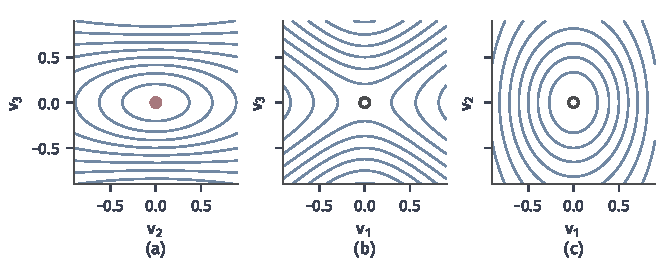
\includegraphics[width=112.0mm]{figures/05-optimization/06-constrained-optimization/matplotlib/mfo-critical-local/figure.pdf}
 \caption{三类驻点附近的局部形状。蓝线是$f(\bm{x}+\bm{v})/\lVert\bm{x}+\bm{v}\rVert_2^2$的等值线，这里的$f$在贯穿例中是二次齐次的，该式等于把$\bm{x}+\bm{v}$归一化后的目标值。$(v_i,v_j)$是切平面坐标。(a)~$\bm{e}_1$，碗形。(b)~$\bm{e}_2$，马鞍形。(c)~$\bm{e}_3$，倒扣的碗。}
 \label{fig:mfo-critical-local}
\end{BookInlineFigure}

\paragraph{曲率与Lagrange函数的Hessian}
为什么约束的弯曲会以乘子的形式进入？设$\bm{c}(t)$是$M$上的曲线，$\bm{c}(0)=\bm{x}$，$\bm{c}'(0)=\bm{v}$。由$h_j(\bm{c}(t))=0$求两次导，得到
\[
 \nabla h_j(\bm{x})^\top\bm{c}''(0)+\bm{v}^\top\nabla^2h_j(\bm{x})\bm{v}=0.
\]

现在求目标沿曲线的二阶导数，它是
\[
 (\bar{f}\circ\bm{c})''(0)=\bm{v}^\top\nabla^2\bar{f}\bm{v}+\nabla\bar{f}^\top\bm{c}''(0).
\]
由式~\eqref{eq:mfo-grad-lagrange}把$\nabla\bar{f}$换成黎曼梯度减去$\bm{J}^\top\bm{\nu}$，再利用上一式把$\nabla h_j^\top\bm{c}''(0)$换掉，就得到
\begin{equation}
 (\bar{f}\circ\bm{c})''(0)=\bm{v}^\top\nabla^2_{\bm{x}\bm{x}}\mathcal{L}(\bm{x},\bm{\nu}(\bm{x}))\bm{v}+\bigl\langle\operatorname{grad}f(\bm{x}),\bm{c}''(0)\bigr\rangle.
 \label{eq:mfo-second-along-curve}
\end{equation}

测地线的加速度是纯法向的，所以取$\bm{c}$为测地线时最后一项为零，左端就是$\langle\bm{v},\operatorname{Hess}f(\bm{x})[\bm{v}]\rangle$。这样切向曲率等于Lagrange函数的Hessian在切空间上的二次型：
\begin{equation}
 \langle\bm{v},\operatorname{Hess}f(\bm{x})[\bm{v}]\rangle=\bm{v}^\top\nabla^2_{\bm{x}\bm{x}}\mathcal{L}(\bm{x},\bm{\nu}(\bm{x}))\bm{v},\qquad\bm{v}\in T_{\bm{x}}M.
 \label{eq:mfo-hess-lagrange}
\end{equation}

球面上核对一下。Lagrange函数的Hessian是
\[
 \nabla^2_{\bm{x}\bm{x}}\mathcal{L}=\bm{A}+2\nu\bm{I}=\bm{A}-q\bm{I},
\]
所以二次型是$\bm{v}^\top\bm{A}\bm{v}-q\lVert\bm{v}\rVert_2^2$，与式~\eqref{eq:mfo-rayleigh-hess}相同。式~\eqref{eq:mfo-second-along-curve}最后那一项在第~\ref{sec:mfo-pullback}节还会用到。

\paragraph{二阶判别}
下面的定理把上述量组织成判别条件，要分清必要与充分。

\begin{theorem}[流形上的最优性条件]
 \label{thm:mfo-optimality}
 设$f$在黎曼流形$M$上二阶连续可微，$\bm{x}^\star\in M$。
 \begin{enumerate}
  \item 若$\bm{x}^\star$是局部极小点，则$\operatorname{grad}f(\bm{x}^\star)=\bm{0}$，且$\operatorname{Hess}f(\bm{x}^\star)$半正定。
  \item 若$\operatorname{grad}f(\bm{x}^\star)=\bm{0}$，且$\operatorname{Hess}f(\bm{x}^\star)$在$T_{\bm{x}^\star}M$上正定，则$\bm{x}^\star$是严格局部极小点。
 \end{enumerate}
\end{theorem}

\begin{proof}
 记指数映射为$\exp_{\bm{x}^\star}$，定义切空间上的函数
 \[
  \phi(\bm{v})=f(\exp_{\bm{x}^\star}(\bm{v})).
 \]

 指数映射在零点的微分是恒等映射，由反函数定理，它把零点的一个邻域微分同胚地映到$\bm{x}^\star$的一个邻域。

 因此$\bm{x}^\star$是$f$的（严格）局部极小点，当且仅当$\bm{0}$是$\phi$的（严格）局部极小点。对单位切向量$\bm{v}$，曲线$\gamma(t)=\exp_{\bm{x}^\star}(t\bm{v})$是测地线，于是
 \[
  \frac{\mathrm{d}}{\mathrm{d}t}\phi(t\bm{v})\Big|_{t=0}=\langle\operatorname{grad}f(\bm{x}^\star),\bm{v}\rangle,
  \qquad
  \frac{\mathrm{d}^2}{\mathrm{d}t^2}\phi(t\bm{v})\Big|_{t=0}=\langle\bm{v},\operatorname{Hess}f(\bm{x}^\star)[\bm{v}]\rangle.
 \]
 这说明$\phi$在零点的欧氏梯度和Hessian正是黎曼梯度和黎曼Hessian。把线性空间上无约束问题的一阶、二阶必要条件和二阶充分条件用到$\phi$上，就得到两个结论。
\end{proof}

两个条件之间有间隙，$\operatorname{Hess}f$半正定但不正定时，定理不作结论。取圆周上的$f(\bm{x})=x_2^3$，在点$(1,0)$处切向坐标为$\theta$，$f=\sin^3\theta$的一阶、二阶导数都为零，二阶必要条件成立，但$\theta<0$时函数值更小，这一点不是局部极小。

半正定也可能来自一整段极小点。取$\bm{A}=\operatorname{diag}(1,1,4)$，圆周$x_3=0$上每一点都是全局极小点，切向曲率有一个零方向，定理第二条不适用，这些点并不是孤立的。

定理也只是局部结论。圆周上的$\cos3\theta+0.3\cos\theta$在$\theta=\pi$附近和$\theta=\pm\pi/3$附近都有严格局部极小，函数值分别约为$-1.30$和$-0.85$，后者满足二阶充分条件却不是全局极小。

Rayleigh商是一个少见的例外，局部极小都是全局极小。设$\bm{x}$是特征向量，特征值$\lambda>\lambda_1$，取$\lambda_1$的单位特征向量$\bm{v}$，它与$\bm{x}$正交，由式~\eqref{eq:mfo-rayleigh-hess}得到
\[
 \langle\bm{v},\operatorname{Hess}f(\bm{x})[\bm{v}]\rangle=\lambda_1-\lambda<0.
\]
所以满足二阶必要条件的驻点只能属于最小特征值。这个结论来自目标的特殊结构，不能推广到一般流形问题。
